% =====================================================================
% THIS FILE IS THE SOURCE. Edit it, then rebuild the PDF with:
%     bash tools/compile.sh Unit_12_Putting_It_Together
% (run from the Course_Rewrite folder; it compiles twice and reports
%  page count, overfull boxes, and em dashes)
%
% Do not edit the PDF directly. Figures are the fig_*.pdf files in this
% folder, regenerated by tools/make_module*_slide_figs.py.
%
% Originally converted from the 15-module draft by a one-shot script now
% parked in tools/one_shot_generators/. Re-running those would discard
% anything you change here, so they are kept out of tools/ on purpose.
% =====================================================================
\documentclass[aspectratio=169]{beamer}
\usetheme{default}
\usefonttheme{professionalfonts}
\usepackage{amsmath, amssymb, amsfonts}
\usepackage{graphicx}
\usepackage{booktabs}
\usepackage{bm}
\usepackage{hyperref}

\mode<presentation> {
    \usetheme{Frankfurt}
    \usecolortheme{default}
}

\newcommand{\xbar}{\bar{x}}
\newcommand{\yhat}{\hat{y}}
\newcommand{\PR}[1]{P(#1)}

\newenvironment{principle}[1]{\begin{block}{\textbf{Principle:} #1}}{\end{block}}
\newenvironment{trap}[1]{\begin{alertblock}{\textbf{Trap:} #1}}{\end{alertblock}}
\newenvironment{practice}[1]{\begin{exampleblock}{\textbf{In practice:} #1}}{\end{exampleblock}}
\newenvironment{interview}[1]{\begin{exampleblock}{\textbf{You may be asked:} #1}}{\end{exampleblock}}
\newenvironment{yourturn}[1]{%
  \setbeamercolor{block title}{fg=white,bg=orange!80!black}%
  \setbeamercolor{block body}{bg=orange!12}%
  \begin{block}{\textbf{Your turn:} #1}}{\end{block}}
\newenvironment{livedemo}[1]{%
  \setbeamercolor{block title}{fg=white,bg=teal!80!black}%
  \setbeamercolor{block body}{bg=teal!12}%
  \begin{block}{\textbf{Live demo:} #1}}{\end{block}}
\newenvironment{llmcheck}[1]{%
  \setbeamercolor{block title}{fg=white,bg=violet!75!black}%
  \setbeamercolor{block body}{bg=violet!10}%
  \begin{block}{\textbf{LLM check:} #1}}{\end{block}}

\title{Putting It Together}
\subtitle{Unit 12: Messy Questions, Answered Out Loud}
\author{Stat 220 \textbar{} Statistics for Data Science}
\date{}

\begin{document}

\begin{frame}
  \titlepage
\end{frame}

% ======================================================================
\section{Why}
% ======================================================================
\begin{frame}{Where this fits}
\begin{itemize}
  \item You now have the tools. This part is about the skill that actually gets tested: taking an
        ambiguous, badly posed question and reasoning through it in front of someone.
  \item Nobody will ask you to derive a $t$-statistic. They will hand you a situation and watch how
        you think.
  \item The good news: the same handful of moves works on almost every question, and you have been
        practicing them all semester.
\end{itemize}
\begin{principle}{what is actually being evaluated}
Not whether you know the formula. Whether you notice what is missing, say what you assume, and know
what would change your answer.
\end{principle}
\end{frame}

\begin{frame}{The whole course on one page}
\begin{center}
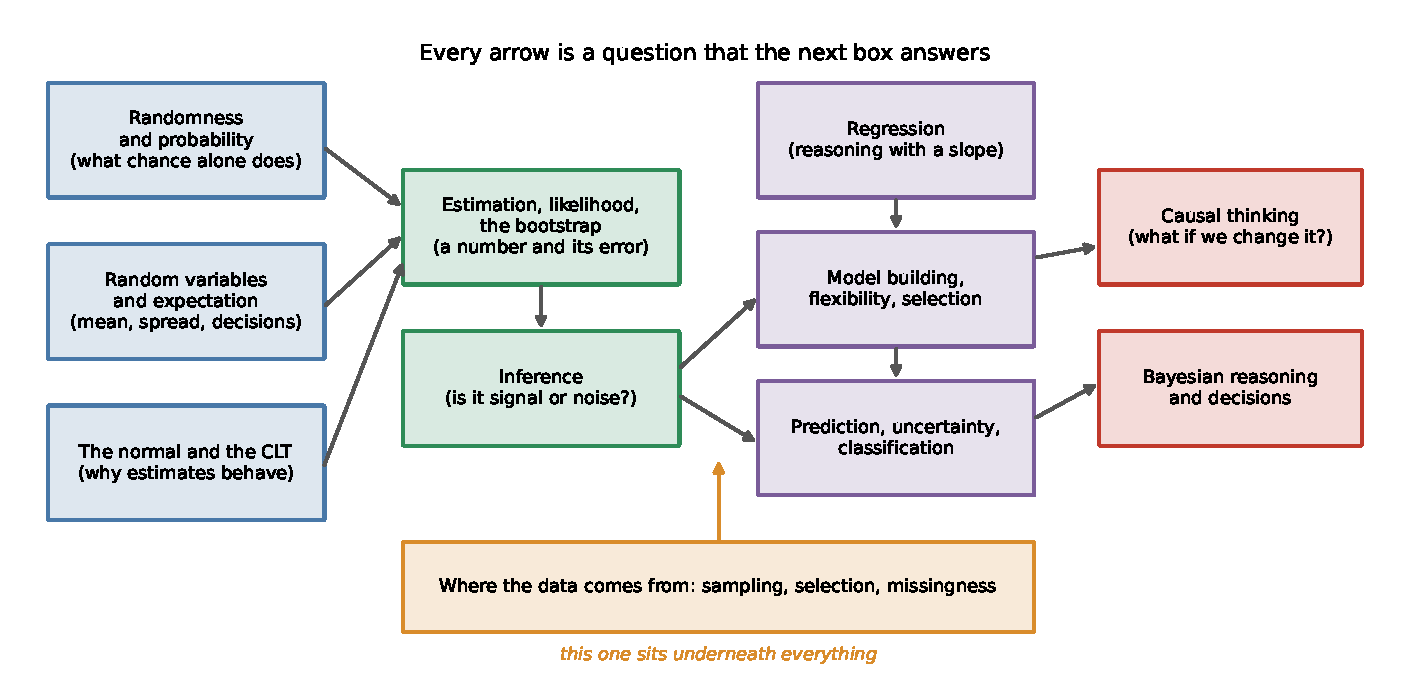
\includegraphics[width=0.95\textwidth]{fig_m15_map.pdf}
\end{center}
\end{frame}

\begin{frame}{Live experiment: the interview bracket}
\begin{livedemo}{two minutes, out loud, no notes}
Pair up. Each pair draws two scenario cards.
\begin{enumerate}
  \item Partner A reads a card. Partner B answers \textbf{out loud for two minutes}. No writing.
  \item Partner A scores using the five-beat rubric on the next slide, one point per beat.
  \item Swap, then the highest scorer from each pair advances.
\end{enumerate}
Semifinalists answer at the front, and the class votes.
\end{livedemo}
\vspace{0.2em}
{\tiny\textit{Materials: printed scenario cards (\texttt{Unit\_12\_Scenario\_Cards.pdf}). Time: 30 minutes for the full bracket.}}
\centering\small The scoring rubric is deliberately not about being right. It is about the shape of
the answer.
\end{frame}

\begin{frame}{The five-beat answer}
Use this structure on any question you are handed:
\begin{enumerate}
  \item \textbf{Clarify.} What decision is this for, and what would count as an answer?
  \item \textbf{State assumptions.} What do you need to be true, and which are you unsure of?
  \item \textbf{Name the approach.} What you would compute, and why that and not something else.
  \item \textbf{Name the traps.} What would make this answer wrong.
  \item \textbf{Say what would change your mind.} What evidence would flip the recommendation.
\end{enumerate}
\begin{principle}{beats 4 and 5 are where candidates separate}
Almost everyone can do the middle. Very few volunteer how their own answer could be wrong, and that
is precisely the mark of someone you can trust with a decision.
\end{principle}
\end{frame}

\begin{frame}{What this unit is}
\begin{itemize}
  \item No new mathematics. Everything here is a tool you already have. The work is choosing which
        one, fast, on a problem stated badly by someone who is not a statistician.
  \item Day 1 builds the reusable answer structure and the checklist. Day 2 runs six full
        scenarios. Day 3 is the bracket, where you do it out loud.
  \item The scenarios come from every unit at once, and none of them announce which unit they came
        from. That is the point.
\end{itemize}
\end{frame}

% ======================================================================
\section{The checklist}
% ======================================================================
\begin{frame}{The universal red-flag checklist}
Run this on \emph{any} number, chart, or claim someone hands you:
\begin{enumerate}
  \item \textbf{Where did this data come from}, and who is missing from it?
  \item \textbf{What is the denominator}, and is it comparable across the groups?
  \item \textbf{How big is the sample}, and how many of the rare thing did we actually see?
  \item \textbf{Where is the uncertainty}? Is there an interval, and is it honest?
  \item \textbf{Was this the only comparison made}, or the winner of many?
  \item \textbf{Is this association being read as a cause}, and what is the comparison group?
  \item \textbf{What would this look like if nothing were happening?}
\end{enumerate}
\end{frame}

\begin{frame}{The end-to-end workflow, consolidated}
\begin{enumerate}
  \item \textbf{Pin the question} to a decision someone will make.
  \item \textbf{Interrogate the data's origin} before you open it.
  \item \textbf{Look at the data} (distributions, missingness, outliers) before modeling.
  \item \textbf{Choose the simplest method the question needs}, and say why.
  \item \textbf{Estimate, with uncertainty}, using a bootstrap when formulas run out.
  \item \textbf{Check the assumption most likely to break}, and check it out of sample.
  \item \textbf{Translate into a recommendation}, with the risk and one caveat.
\end{enumerate}
\centering\small Every module contributed one line to this list.
\end{frame}

% ======================================================================
\section{Scenarios}
% ======================================================================
\begin{frame}{Scenario 1: the metric that jumped}
\textbf{They say:} ``Signups are up 22\% this week. The new homepage is working. Roll it out
everywhere.''
\vspace{0.4em}

\begin{yourturn}{two minutes, out loud}
What do you ask, what do you compute, and what would make you say yes?
\end{yourturn}
\end{frame}

\begin{frame}{Scenario 1: a strong answer}
\begin{itemize}
  \item \textbf{Clarify:} 22\% of what base, over what window, and compared to which period?
  \item \textbf{Assumptions:} that nothing else changed that week. Check holidays, a marketing
        push, a tracking change, and last year's same week.
  \item \textbf{Approach:} if the homepage was launched to everyone at once, there is no control
        group and no causal estimate. Look for a staged rollout or a holdout region for a
        difference-in-differences comparison.
  \item \textbf{Traps:} week-to-week noise on a small base, a definition change, regression to the
        mean after a bad week, and the seasonality that affects everyone.
  \item \textbf{Changes my mind:} a randomized holdout showing the same lift.
\end{itemize}
\end{frame}

\begin{frame}{Scenario 2: the impressive model}
\textbf{They say:} ``Our new churn model is 96\% accurate and its AUC is 0.99. Can we start acting
on it Monday?''
\vspace{0.4em}

\begin{yourturn}{two minutes, out loud}
What is your first reaction, and what three things do you check before Monday?
\end{yourturn}
\end{frame}

\begin{frame}{Scenario 2: a strong answer}
\begin{itemize}
  \item \textbf{First reaction:} suspicion, not celebration. If churn is 4\%, predicting ``nobody
        churns'' scores 96\%, and an AUC of 0.99 on a human behavior problem usually means leakage.
  \item \textbf{Check 1:} the base rate and the trivial baseline. \textbf{Check 2:} whether any
        feature is knowable only \emph{after} the outcome. \textbf{Check 3:} precision and recall
        at the threshold we will actually use.
  \item \textbf{Then the real question:} what action follows a flag, what does a false alarm cost,
        and what does a miss cost? That gives the threshold.
  \item \textbf{Changes my mind:} clean performance on a time-split holdout with no post-outcome
        features.
\end{itemize}
\end{frame}

\begin{frame}{Scenario 3: the subgroup discovery}
\textbf{They say:} ``The campaign didn't work overall, but it was hugely effective for women aged
35 to 44 in the Midwest. Let's target them.''
\vspace{0.4em}

\begin{yourturn}{two minutes, out loud}
Is this a finding? What would you need to believe it?
\end{yourturn}
\end{frame}

\begin{frame}{Scenario 3: a strong answer}
\begin{itemize}
  \item This is a \textbf{multiple comparisons} problem. With a dozen
        demographic splits there are hundreds of subgroups, and the best one always looks
        impressive.
  \item Ask: was this subgroup specified \emph{before} the analysis? How many were examined? What is
        the sample size inside it?
  \item Expect \textbf{regression to the mean}: the effect will shrink substantially on new data,
        even if something real is there.
  \item \textbf{What would convince me:} the same subgroup effect replicating in a fresh campaign,
        preregistered.
\end{itemize}
\begin{practice}{the line to remember}
``Subgroup findings are hypotheses, not conclusions. I would treat this as a candidate to test, not
a result to act on.''
\end{practice}
\end{frame}

\begin{frame}{Scenario 4: the executive summary}
\textbf{They say:} ``Customers who use our mobile app spend 3 times more. We should push everyone
to install the app.''
\vspace{0.4em}

\begin{yourturn}{two minutes, out loud}
What is wrong, and what would you propose instead?
\end{yourturn}
\end{frame}

\begin{frame}{Scenario 4: a strong answer}
\begin{itemize}
  \item \textbf{Selection, not effect.} People who install the app were already your most engaged
        customers. The app is a marker of loyalty at least as much as a cause of it.
  \item \textbf{Reverse causation is live too:} heavy spenders install the app \emph{because} they
        shop often.
  \item \textbf{Proposal:} randomize an install prompt across a holdout, or use a staged rollout by
        region, and measure the change in spending rather than its level.
  \item \textbf{The honest interim answer:} adjusting for prior spending and tenure shrinks the
        3-times gap substantially, and whatever remains is still not an effect.
\end{itemize}
\end{frame}

\begin{frame}{Scenario 5: the survey}
\textbf{They say:} ``Our NPS survey came back at 42, up from 38. Customer satisfaction is
improving.''
\vspace{0.4em}

\begin{yourturn}{two minutes, out loud}
What do you need to know before you believe the four-point move?
\end{yourturn}
\end{frame}

\begin{frame}{Scenario 5: a strong answer}
\begin{itemize}
  \item \textbf{How many responded, and out of how many asked?} A 4-point move on 200 responses is
        well inside noise.
  \item \textbf{Did the responding population change?} If the survey went out after a service
        outage last quarter and not this one, you are comparing different people.
  \item \textbf{Did the instrument change?} Question wording, placement, and timing all move scores
        without moving satisfaction.
  \item \textbf{What I would do:} attach an interval to both numbers, compare responders to
        non-responders on the variables we do have, and corroborate with behavior, such as renewal
        and usage.
\end{itemize}
\end{frame}

\begin{frame}{Scenario 6: the forecast}
\textbf{They say:} ``The model predicts \$4.2M in revenue next quarter. Put it in the board deck.''
\vspace{0.4em}

\begin{yourturn}{two minutes, out loud}
What do you add before that number goes in front of the board?
\end{yourturn}
\end{frame}

\begin{frame}{Scenario 6: a strong answer}
\begin{itemize}
  \item \textbf{An interval, sized from real out-of-sample errors}, not from the training fit. A
        point forecast with no range is half an answer.
  \item \textbf{Which layer of error dominates:} noise, estimation, model structure, or shift? For a
        quarterly forecast in a changing market, shift usually dominates, and no in-sample statistic
        warns you.
  \item \textbf{Whether we are extrapolating:} is next quarter inside the range of conditions the
        model was fit on?
  \item \textbf{One sentence of caveat:} the conditions under which this number should not be
        trusted.
\end{itemize}
\begin{principle}{what to hand a board}
The point, the range, the dominant source of error, and the one thing that would make it wrong.
\end{principle}
\end{frame}

% ======================================================================
\section{Communicating}
% ======================================================================
\begin{frame}{Scenario 7: the model that decides about people}
\textbf{They say:} ``Our hiring model is 88\% accurate at predicting who will be a top performer.
Let's use it to screen applications.''
\vspace{0.4em}

\begin{yourturn}{two minutes, out loud}
What do you ask, what could go wrong, and what would you need before this touches a real
applicant?
\end{yourturn}
\end{frame}

\begin{frame}{Scenario 7: a strong answer}
\begin{itemize}
  \item \textbf{The label:} ``top performer'' is a manager's rating, a proxy carrying whatever
        biases that manager had. The model predicts the rating, not the performance.
  \item \textbf{The sample:} it only observes people who were \emph{hired}. Strong candidates the
        old process rejected are invisible, so the model learns the old process.
  \item \textbf{The metric:} 88\% accuracy means nothing without the base rate. If 85\% of hires
        are rated acceptable, the model is barely beating ``say yes.''
  \item \textbf{Before deployment:} the base rate, precision and recall at the operating
        threshold, error rates broken out across groups, and a human in the loop.
\end{itemize}
\end{frame}

\begin{frame}{Scenario 8: the number with no error bar}
\textbf{They say:} ``Customer lifetime value is \$1,840. I've put it in the pricing model.''
\vspace{0.4em}

\begin{yourturn}{two minutes, out loud}
Where did that number come from, and what are the three things you check before pricing depends on
it?
\end{yourturn}
\end{frame}

\begin{frame}{Scenario 8: a strong answer}
\begin{itemize}
  \item \textbf{Mean or median?} Lifetime value is heavily right-skewed. If \$1,840 is a mean, a
        handful of whales are setting your prices for everyone.
  \item \textbf{Which customers?} Almost certainly the ones who have already churned, since only
        they have a complete lifetime. That is survivorship in reverse: your best customers are
        excluded precisely because they are still here.
  \item \textbf{How wide is the interval?} A bootstrap on a skewed quantity like this is often
        embarrassingly wide, and pricing built on a point estimate inherits all of that.
  \item \textbf{What I would report:} median and mean, an interval on each, and a segment
        breakdown, because one number for all customers is the actual error here.
\end{itemize}
\end{frame}

\begin{frame}{Translating for a non-technical audience}
\begin{itemize}
  \item \textbf{Lead with the decision}, not the method. ``Ship it'' or ``do not ship yet, and here
        is what would settle it.''
  \item \textbf{Quantify the risk in their units:} dollars, customers, hours, not $p$-values.
  \item \textbf{Use natural frequencies:} ``about 6 of every 100'' beats ``a 6\% rate,'' and both
        beat ``an 18\% relative increase.''
  \item \textbf{Give one caveat, not five.} The most likely way to be wrong, in one sentence.
\end{itemize}
\begin{trap}{two opposite failures}
Drowning the room in caveats is as useless as hiding all of them. Pick the one that could change the
decision.
\end{trap}
\end{frame}

\begin{frame}{When you do not know}
\begin{itemize}
  \item Say so, then keep going: ``I do not know, but here is how I would find out.'' That answer
        scores well, and pretending scores zero.
  \item Reason out loud. The interviewer is watching the process, not waiting for a number.
  \item Anchor on what you do know: the base rate, the sample size, the comparison group, what
        chance alone would produce.
\end{itemize}
\begin{principle}{the honest default}
``It depends'' is a fine start, as long as the next sentence says \emph{on what}, and the one after
that says what you would check first.
\end{principle}
\end{frame}

% ======================================================================
\section{LLM check}
% ======================================================================
\begin{frame}{LLM check: mistake or not? (1 of 2)}
\begin{llmcheck}{we gave an LLM a full interview question}
\textbf{We told it:} ``Our conversion rate dropped from 4.1\% to 3.8\% last month. What happened?''
\\[4pt]
\textbf{It answered:} ``A 0.3-point drop is a 7.3\% decline in conversion. Likely causes include
increased competition, seasonal effects, and site performance issues. I would recommend auditing
your checkout flow and running a competitor analysis.''
\end{llmcheck}
\vspace{0.2em}
\centering\small Mistake, or no mistake?
\onslide<2->{%
\begin{trap}{verdict: mistake}
It jumped straight to explanations without asking whether there is anything to explain. No sample
size, no interval, no check on whether tracking or the definition changed. It is generating
plausible stories for what may be noise.
\end{trap}}
\end{frame}

\begin{frame}{LLM check: mistake or not? (2 of 2)}
\begin{llmcheck}{same question, a different answer}
\textbf{We told it:} ``Our conversion rate dropped from 4.1\% to 3.8\% last month. What happened?''
\\[4pt]
\textbf{It answered:} ``First, how many visitors? At 5{,}000 a month that difference is well within
noise, and at 5 million it is not. Before looking for causes I would check whether tracking or the
conversion definition changed, whether traffic mix shifted, and how this month compares to the same
month last year. If it survives all that, then we look for causes.''
\end{llmcheck}
\vspace{0.2em}
\centering\small Mistake, or no mistake?
\onslide<2->{%
\begin{principle}{verdict: no mistake}
Sample size first, instrument second, mix third, causes last. That ordering is the entire course in
four sentences.
\end{principle}}
\end{frame}

% ======================================================================
\section{Consolidate}
% ======================================================================
\begin{frame}{The whole workflow, in order}
\small
\begin{enumerate}
  \item \textbf{Pin the question} to a decision somebody will make.
  \item \textbf{Interrogate the data's origin} before you open it: population, frame, who is missing.
  \item \textbf{Look at the data}: distributions, missingness, outliers, and what one observation is.
  \item \textbf{Choose the simplest method the question needs}, and say why that one.
  \item \textbf{Estimate with uncertainty}, using a bootstrap when no formula applies.
  \item \textbf{Check the assumption most likely to break}, out of sample.
  \item \textbf{Translate into a recommendation} with the risk and one caveat attached.
\end{enumerate}
\end{frame}

\begin{frame}{The master trap list (1 of 2)}
\begin{trap}{the ones that come up most}
\begin{itemize}\small
  \item Ignoring the base rate after a positive test or a model flag.
  \item Reporting accuracy on imbalanced data, or a rate with no denominator.
  \item Quoting a relative change with no absolute change.
  \item Confusing $\PR{A \mid B}$ with $\PR{B \mid A}$.
  \item Reporting a point estimate with no interval, or an interval that is too narrow.
  \item Treating the winner of many comparisons as a discovery.
  \item Counting rows instead of independent units.
\end{itemize}
\end{trap}
\end{frame}

\begin{frame}{The master trap list (2 of 2)}
\begin{trap}{the ones that end careers}
\begin{itemize}\small
  \item Reading a regression coefficient as the effect of an intervention.
  \item Controlling for a collider or a mediator.
  \item Judging a model on training data, or tuning on the test set.
  \item Believing a near-perfect model instead of hunting for leakage.
  \item Treating a big sample as a representative one.
  \item Dropping missing rows without asking why they are missing.
  \item Extrapolating past the data, and assuming the future matches the past.
\end{itemize}
\end{trap}
\end{frame}

\begin{frame}{The final question bank (1 of 2)}
Answer each in two minutes, out loud, using the five beats.
\begin{enumerate}\small
  \item A test is 99\% accurate and you tested positive for a rare disease. Now what?
  \item Our A/B test shows a 40\% lift with $p = 0.04$ on 500 users. Do we ship?
  \item Why is a prediction interval wider than a confidence interval?
  \item Users of feature X retain better. Should we push everyone onto it?
  \item Our model is 96\% accurate. Are you impressed?
  \item How would you put error bars on a forecast?
  \item Should you control for everything you have? Explain.
  \item Our data is skewed. Can we still use a $t$-test?
\end{enumerate}
\end{frame}

\begin{frame}{The final question bank (2 of 2)}
\begin{enumerate}\small
  \setcounter{enumi}{8}
  \item We have 12 million rows. Do we still need to think about sampling?
  \item How would you set the threshold on a fraud model?
  \item Our best rep slumped last quarter. Did the new comp plan fail?
  \item A subgroup shows a huge effect. Do we target it?
  \item Explain the bootstrap in thirty seconds.
  \item What would you check before explaining a spike in a dashboard?
  \item How do you know you are not overfitting?
  \item What is the single most important question to ask about any dataset?
\end{enumerate}
\end{frame}

\begin{frame}{The mastery checklist for the whole course}
You are ready when you can, without notes:
\begin{itemize}
  \item say what chance alone would produce, before explaining any pattern
  \item attach an honest interval to any estimate, formula or not
  \item translate any accuracy claim into the conditional probability someone needs
  \item tell an association from a causal claim, and name what design would earn the second
  \item judge a model on data it has never seen, and say what would break it
  \item trace any dataset back to the process that made it, and name who is missing
  \item turn all of that into a recommendation with a stated risk and one caveat
\end{itemize}
\end{frame}

\begin{frame}{Running the bracket (logistics)}
\begin{itemize}
  \item \textbf{Round 1 (pairs, 10 min).} Everyone answers one card, partner scores the five
        beats. Swap. Higher score advances.
  \item \textbf{Round 2 (fours, 10 min).} Winners pair off, and the two losers score.
  \item \textbf{Semifinals and final (front of room).} Two minutes each, class votes with the
        rubric, not on charisma.
  \item \textbf{The rule that matters:} nobody may say ``run a $t$-test'' without saying what
        would make the test inappropriate.
\end{itemize}
\begin{principle}{what wins}
Not the most confident answer. The one that names its own assumptions and says what would change
its mind.
\end{principle}
\end{frame}

\begin{frame}{What you should be able to do with software}
\small
Nobody is asking you to memorize syntax. You are expected to know \emph{which} procedure the
question calls for, what to hand it, and what the output means. With an AI assistant open, you
should be able to produce any of these and defend the result.
\begin{center}\footnotesize
\begin{tabular}{p{0.44\textwidth} p{0.46\textwidth}}
\toprule
\textbf{You should be able to} & \textbf{What you would reach for} \\
\midrule
Everything from Units 1 through 11, on demand & you should not need to be told which \\
Load, inspect, and audit a new dataset & \texttt{read\_csv}, \texttt{describe}, \texttt{isna} \\
Compare two groups honestly & \texttt{ttest\_ind}, plus an interval \\
Fit and validate a model & \texttt{cross\_val\_score} inside a pipeline \\
Attach an interval to any estimate & bootstrap, or held-out residuals \\
Turn a prediction into a decision & expected cost over the predictive distribution \\
Say what the analysis cannot support & no library for this one \\
\bottomrule
\end{tabular}
\end{center}
\vspace{0.2em}
\centering\small
If you cannot say what the output means, the fact that you produced it is worth nothing.
\end{frame}

\begin{frame}{The last slide}
\begin{itemize}
  \item Computation is cheap and getting cheaper. A model can be fit by anyone, in one line, in
        seconds.
  \item What does not get cheaper is knowing which question to ask, which number is meaningless,
        and when the confident answer on the screen is wrong.
  \item That judgment is the job. It is what you have been building all semester, and it is what
        every one of those interview questions is really testing.
\end{itemize}
\begin{principle}{the whole course, in one sentence}
Anyone can produce a number. You have been trained to ask what would have to be true for that
number to mean anything.
\end{principle}
\end{frame}

\end{document}
